\chapter{\gls{PNG}}

\section{\gls{W3C} international standard}
\begin{itemize}
\item Developed by the \href{https://www.w3.org/}{W3C}, \gls{PNG} \cite{roelofs1999png} is
  supported by all Web browsers, and most image viewers.
\end{itemize}
%\vspace{-4ex}
\begin{center}
  \href{https://upload.wikimedia.org/wikipedia/commons/0/05/CT_of_a_normal_abdomen_and_pelvis%2C_coronal_plane_79.png}{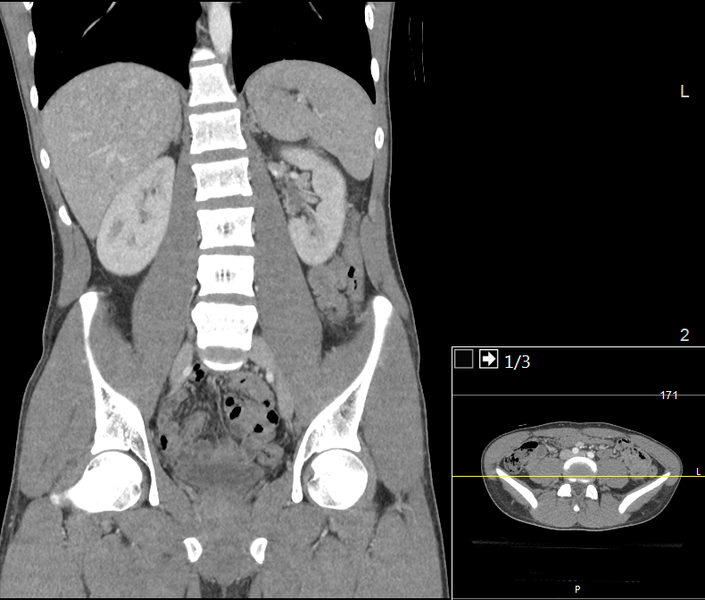
\includegraphics[width=6cm]{CT_example}}\\
     (click on the image)
\end{center}

\section{Raster graphics file format}
\begin{itemize}
\item Up to ($2^{32}-1$)x($2^{32}-1$) pixels, efficiently represented
  (lossless compression with DEFLATE \cite{deutsch1996deflate}).
\item Pixels can be gray-scale (1 channel) or color
  \popup{\gls{RGBA}}{Red, Green, Blue, and Alpha (transparency)
    channels. The alpha-channel is optional.} (4 channels).
\end{itemize}
\vspace{-4ex}
\begin{center}
  \href{https://en.wikipedia.org/wiki/Raster_graphics}{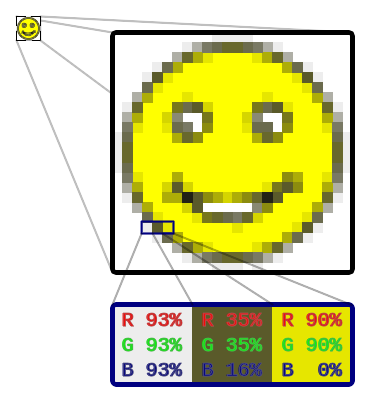
\includegraphics[width=5cm]{RGB-raster-image}}
\end{center}

\section{8 and 16 bits/channel}
\begin{itemize}
\item In gray-scale image:
  \begin{center}
    \begin{tabular}{c|c}
      & Number of \\
      Bits/channel & gray-scale values \\
      \hline
      8 & $2^8=256$ \\
      16 & $2^{16}=65536$
    \end{tabular}
  \end{center}
\item These pixel ``depth'' should be fine for most medical images.
  \begin{center}
    \href{https://www.fastcompression.com/blog/jpeg2000-applications-part1.htm}{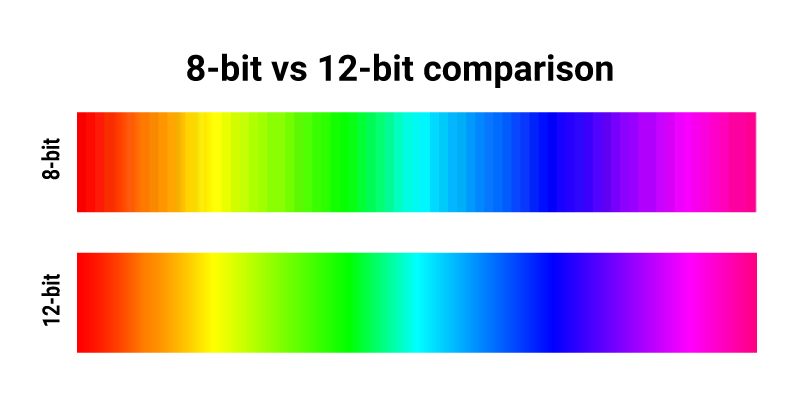
\includegraphics[width=8cm]{8bit_vs_12bit}}
  \end{center}
\end{itemize}

\section{Progressive rendering}
\begin{itemize}
\item Optional. Pixels are displayed using the Adam7 algorithm.
\end{itemize}
\begin{center}
  \href{https://upload.wikimedia.org/wikipedia/commons/2/27/Adam7_passes.gif}{
\includegraphics[width=5cm]{Adam7_passes-0}} \\
  (Click in the image)
\end{center}
  
\section{\popup{Animated}{Also called ``motion''.} PNG}
\begin{itemize}
\item A \gls{APNG} is sequence of images in a \gls{PNG} file.
\end{itemize}
\begin{center}
  \href{https://commons.wikimedia.org/wiki/Category:Animated_PNG_files#/media/File:201805_human_skeleton_anim.png}{\includegraphics[width=5cm]{human_skeleton_anim}} \\
  (Click in the image)
\end{center}

\section{Image metadata}
\begin{itemize}
\item \gls{PNG} images can store metadata:
  \begin{center}
    \begin{tabular}{l|l}
      Keyword & Meaning\\
      \hline
      Title & Short (one line) title or caption for image \\
      Author & Name of image's creator \\
      Description & Description of image (possibly long) \\
      Copyright & Copyright notice \\
      Creation Time & Time of original image creation \\
      Software & Software used to create the image \\
      Disclaimer & Legal disclaimer \\
      Warning & Warning of nature of content \\
      Source & Device used to create the image \\
      Comment & Miscellaneous comment; conversion from GIF comment
    \end{tabular}
  \end{center}
\end{itemize}

\begin{itemize}
\item
  \href{https://github.com/vicente-gonzalez-ruiz/medical_imaging/blob/main/notebooks/PNG_add_metadata.ipynb}{Here}
  there is an example that shows and modifies the metadata in a PNG
  image.
\end{itemize}